
Se plantea el siguiente circuito equivalente:

%circuito equivalente Inductancia
\begin{figure}[H]
\centering
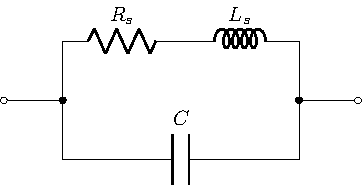
\includegraphics[width=6cm,height=4cm]{Ejercicio_1(Germo)/Circuitos/circuito_equivalente_inductancia.pdf}
\label{fig:circuito_equivalente_inductancia}
 \begin{center}
     \begin{table}[H]
				1K    & 0.480         & 16.6	& 0.18 		& 3.02  & 86.0     \\
